\chapter{Fejlesztői dokumentáció} % Developer guide
\label{ch:impl}

\section{A NES felépítése}

\begin{figure}[H]
	\centering
	\includegraphics[scale=0.22]{mobo.jpg}
	\caption{A NES alaplapja}
\end{figure}

A NES emulációjához a következő komponenseket kell megismernünk és megvalósítanunk:

\begin{compactdesc}
	\item[Ricoh RP2A03:] A hangchipet és központi feldolgozóegységet tartalmazó integrált áramkör. Utóbbi nem más, mint az Apple II-ben és Commodore 64-ben használt 8-bites MOS Technology 6502.
	\item[Ricoh RP2C02:] A képfeldolgozó egység, rövid nevén PPU (Picture Processing Unit).
	\item[NROM és UNROM:] 
	Az emulátor által támogatott két kazettatípus.
	\item[Sztenderd NES kontroller:] 
	A konzol alapértelmezett beviteli eszköze.
\end{compactdesc}

\section{Órajel-frekvenciák}
A párhuzamosan működő komponenseket az órajelek hangolják össze. Az órajel-frekvencia határozza meg, hogy egy másodperc alatt hány atomi műveletet végez el egy komponens.
Minden komponens rendelkezik egy saját órajelfrekvenciával, amit egy központi órajelből származtatnak.

\begin{itemize}
	\item Központi órajel-frekvencia: $ f = \frac{236.25\;MHz}{11} \sim 21.477272\; MHz $
	\item CPU órajel-frekvencia: $ \frac{f}{12} \sim 1.789773 \; MHz  $
	\item PPU órajel-frekvencia: $ \frac{f}{4}  \sim 5.369318 \; MHz $
\end{itemize}

\section{A központi feldolgozóegységhez kapcsolódó fogalmak}

\begin{note}
	A hexadecimális értékeket \textbf{\$} prefix-el jelölöm.
\end{note}

\subsection{Opkód} 
Egy opkód a 6502 esetében csupán egyetlen bájt, amiből az utasításdekódoló egyértelműen meg tudja határozni a végrehajtandó utasítást és annak címzési módját.
Ezt a hozzárendelést az opkódmátrix írja le. Az emulációhoz emellett azt is tárolni kell az opkódmátrixban, hogy a végrehajtandó művelet hány központi órajel alatt fejeződik be, ugyanis ebből tudjuk megállapítani, hogy a processzor utasításával párhuzamosan hány órajelet kell kapnia a képfeldolgozónak. 

\begin{figure}[H]
	\centering
	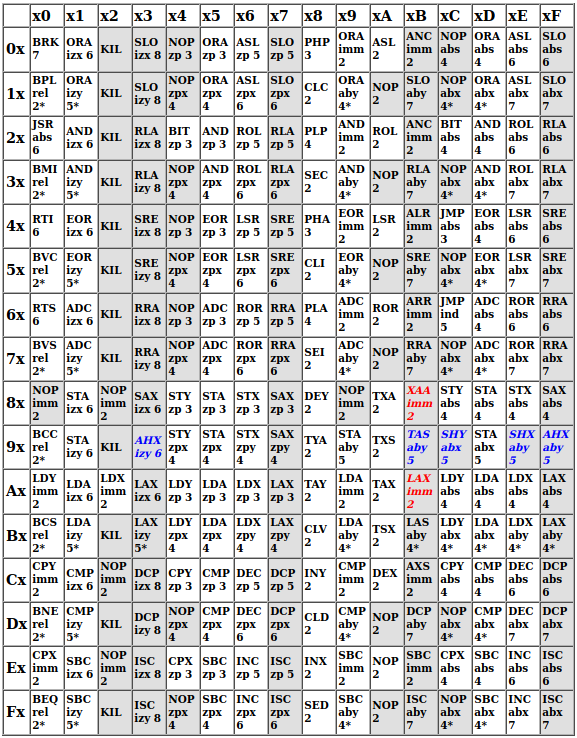
\includegraphics[scale=0.65]{opcodes.png}
	\caption{A 6502 opkódmátrixa}
	\label{fig:opcodes}
\end{figure}

Ha meg szeretnénk találni egy adott opkódhoz a hozzá tartozó információt, akkor szükségünk lesz az opkód hexadecimális alakjára, ami legfeljebb két számjegyű lehet. A nagyobb helyiértékű számjegy a keresett cella sorát, a kisebbik pedig az oszlopát írja le. Példaként a \ref{fig:opcodes} ábrán láthatjuk, hogy a \textbf{\$30} opkódhoz a BMI utasítás tartozik relatív címzéssel.
Azok az opkódok csillaggal vannak jelölve, amiknek futási ideje csak végrehajtás során dönthető el, az aktuális argumentumok alapján.
A szürkével jelölt opkódokhoz hivatalosan nincs utasítás rendelve. 
Ezeket a nem dokumentált, "illegális" opkódokat a processzor későbbi 
verzióinak hagyták fent. A tervezők nem tiltották meg azonban ezeknek a használatát, 
egyszerűen csak nem definiálták a viselkedésüket. Ennek ellenére több olyan illegális opkód is belekerült a dizájnba, ami később hasznosnak bizonyult. A fejlesztők próbálkozások útján
felfedezték, hogy melyek azok az opkódok, amiknek a viselkedése determinisztikus és néhány speciális feladat esetén érdemes őket használni.
Ritka ugyan, de van olyan játék, ami ezeket az opkódokat is használja, így ajánlott ezeket is emulálni.

\subsection{Regiszterek}
A regiszter a processzor leggyorsabban elérhető memóriája.
A gyártási költségek alacsonyan tartása végett csak 6 regiszter került a processzorba.

\begin{compactdesc}
	\item[A:] Akkumulátor, az aritmetikai műveletek eredményei ebbe kerülnek.
	\item[X és Y:] 
	Index regiszterek, indirekt címzésnél használjuk őket.
	Ciklusok esetén a ciklusváltozót érdemes ezekben tárolnunk.
	\item[S:] 
	Verem mutató. A verem tetejének a kezdőcímtől vett eltolását tárolja.
	\item[P:]
	Státusz regiszter, ami 7 darab flag bitet tárol.
	\item[PC:]
	Programszámláló. A következő opkód memóriacímét tárolja.
	A többi regiszterrel ellentétben ez nem 8, hanem 16 bites.
	Ebből következik, hogy a processzor címtartományának mérete 64 KiB.
\end{compactdesc}


\subsection{Memórialap}
Az $i$. lap egy 256 bájtos egybefüggő memóriarész, ami a $ [i \cdot \$100, \: (i+1) \cdot \$100) $ címtartományon helyezkedik el.

\subsection{Hívási verem}
Az egymásba ágyazott eljárásokat a processzor hardveresen támogatja, amihez egy vermet használ.
A verem az 1. lapon található, és a kisebb címek felé nő.
Eljárás hívásakor a verem tetejére kerül az aktuális programszámláló értéke, 
visszatéréskor pedig a veremről levett címre állítjuk be a programszámláló értékét.

\subsection{Megszakítás}
A komponensek kommunikációjának egyik módja a hardveres megszakítás.
A 6502 chip egy darab maszkolható \emph{(IRQ)} és egy nem maszkolható \emph{(NMI)} megszakítási lábbal rendelkezik.
A megszakítási vektorral a program megszabhatja, hogy adott megszakítás esetén a vezérlés melyik szubrutinhoz ugorjon. Például ha van egy szubrutin, amit NMI esetén futtatni szeretnénk, akkor a \textbf{\$FFFA} és a \textbf{\$FFFB} címekre be kell írni a szubrutin címét, a kevésbé szignifikáns bájttal kezdve.
A program dönthet úgy, hogy a maszkolható megszakítást figyelmen kívül hagyja, ehhez a megfelelő flag-et be kell állítania a státusz regiszterben. A nem maszkolható megszakítást esetén erre nincsen lehetőség, a végrehajtás mindenképpen a kezelő szubrutinhoz ugrik.
A nem maszkolható lábhoz a képfeldolgozó, a maszkolhatóhoz a hangchip van kötve.

\subsection{Opkód argumentumok fajtái}

\begin{figure}[H]
	\centering
	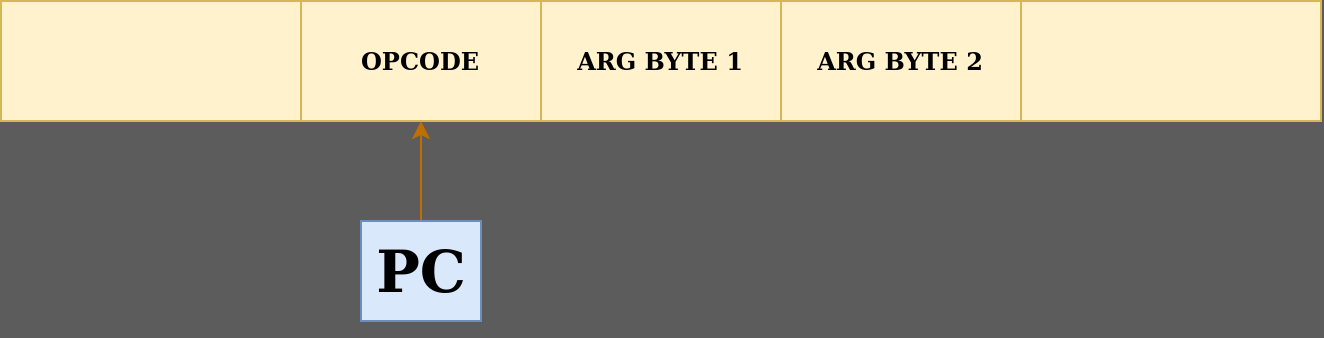
\includegraphics[scale=0.25]{opcode.png}
	\caption{Opkód argumentumainak helye}
\end{figure}

\begin{compactitem}
	\item Abszolút memóriacím (16 bit)
	\item Eltolást leíró bájt
	\item Közvetlen operandusként szolgáló bájt
\end{compactitem}

\subsection{Címzési módok}

Egy opkód után azoknál a címzési módoknál áll argumentum, amiknél a művelet elvégzéséhez 
szükséges operandus nem regiszterben, hanem a memóriában van. A címzési módok azt határozzák meg, hogy az argumentumból hogyan kell kiszámolni az operandus effektív 16 bites memóriacímét. A címzési mód mögött álló zárójelben az opkódmátrixbeli név (amennyiben van) és az argumentum bájtok száma található.  


\begin{description}
	\item[Akkumulátor mód (0):] nincs argumentum, az utasítás az \textbf{A} regiszter értékét módosítja.
	\item[Azonnali mód (imm, 1):] az utasítás operandusa maga az argumentum. Jele: \#
	\newline
	Példa: az LDA \#\$0 utasítás nullára állítja az \textbf{A} regisztert.
	\item[Abszolút mód (abs, 2):] a paraméter az operandus effektív címe.
	\item[0. lap mód (zp, 1):] A CPU kevés regiszterét azzal ellensúlyozták, hogy ennek a speciális módnak köszönhetően a nulladik lapot hatékonyabban lehet címezni, mint a többit. 
	Mivel a 0. lap mérete 256 bájt, ezért teljes cím helyett elég egyetlen bájt a címzéséhez.
	A kisebb paraméter gyorsabban beolvasható és egyúttal a kódméretet is csökkenti.
	\item[Indexelt 0. lap mód (zpx, zpy, 1):]
	Hasonlóan most is csak a 0. lapot tudjuk címezni, de az argumentumhoz hozzáadjuk valamelyik index regiszter értékét.
	Az operandus címének kiszámítása: $ (arg1 + index) \mod 256 $
	\item[Indexelt abszolút mód (abx, aby, 2):] Az argumentum egy teljes memóriacím, amihez hozzáadjuk a megadott index regiszter értékét. 
	\item[Implicit mód (0):] nincs szükség argumentumra, mert az utasítás regiszterekkel dolgozik.
	\item[Relatív mód (rel, 1):] Az elágazási utasítások használják ezt a címzési módot. Elágazásoknál ha a feltétel teljesül, akkor az argumentummal el kell tolni a programszámlálót.
	\item[Indirekt mód (ind, 2):] 
	Erre a címzési módra a JMP utasításnál van szükség.
	A két argumentum bájt együtt egy teljes memóriacímet alkot, legyen ez \emph{m}.
	Az operandus címét innen kell kiolvasnunk, vagyis a következőképpen kapjuk meg: $ (read(m+1) << 8) \;\; | \;\; read(m) $ 
	\item[Indexelt indirekt mód (izx, 1):]
	Az X regisztert összeadjuk az argumentummal, így egy 0. lapon található címet kapunk.
	Ezen címen az alsó, a következőn pedig a felső 8 bitje található az operandus effektív memóriacímének.
	\begin{figure}[H]
		\centering
		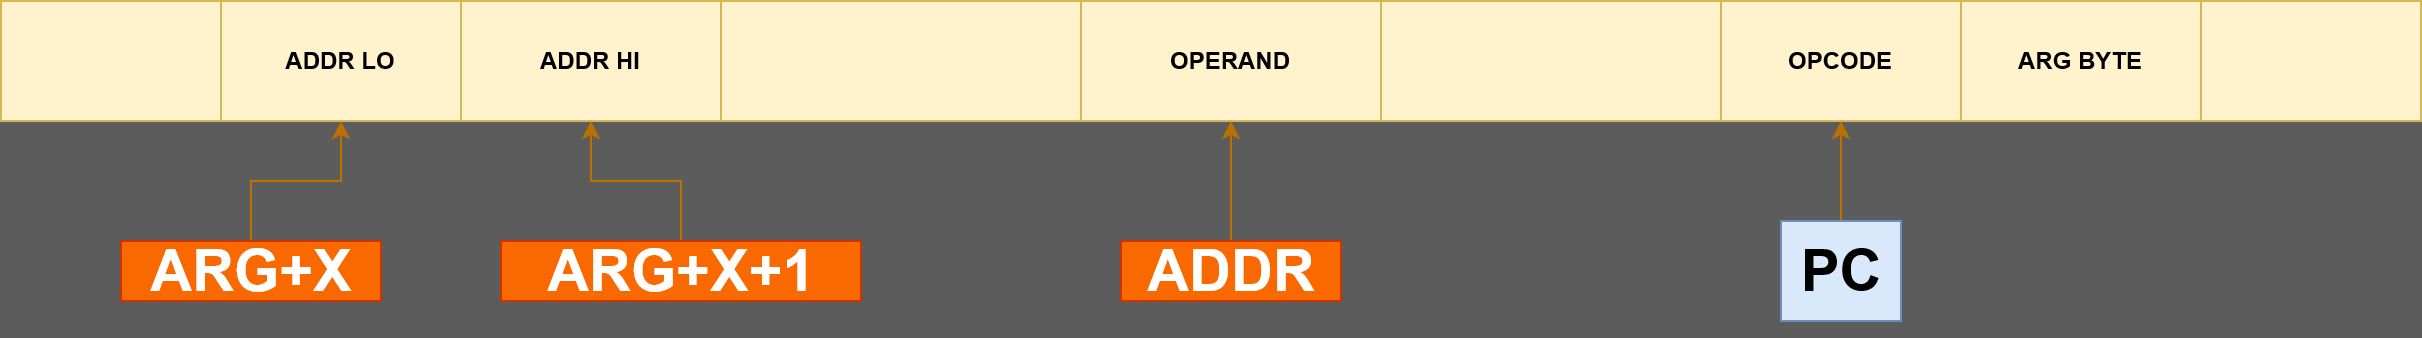
\includegraphics[width=1.1\textwidth,height=70px]{indexed_indirect.png}
		\caption{Indexelt indirekt címzés}
	\end{figure}
	\item[Indirekt indexelt mód (izy, 1):]
	Az argumentum egy 0. lapon található címre mutat, amit ha összeadunk az Y regiszter értékével, akkor megkapjuk az operandus effektív címét. 
	
	
	
\end{description}

Az \textbf{abx}, \textbf{aby} és \textbf{izy} indexelt címzési módok és bizonyos utasítások kombinációjánál előfordulhat, hogy a végleges operandus cím és az indexelés előtt álló cím különböző memórialapra esik. Ebben az esetben 1 órajelciklussal tovább tart az utasítás végrehajtása.

\subsection{Memóriatérkép}

A memóriatérkép leírja a címtér felosztását a komponensek között.
A memóriatérképből meg tudjuk állapítani, hogy egy adott címen található bájt kiolvasásához vagy írásához melyik komponens hardveres logikáját kell alkalmazni.

\begin{table}[H]
	\centering
	\begin{tabular}{ | l | l | }
		\hline
		Tartomány & Eszköz \\
		\hline			
		$ \$0000 - \$07FF $ & CPU RAM \\
		$ \$0800 - \$1FFF $ & CPU RAM tükrözése \\
		$ \$2000 - \$2007 $ & PPU regiszterek \\
		$ \$2008 - \$3FFF $ & PPU regiszterek tükrözése \\
		$ \$4000 - \$4017 $ & APU és IO regiszterek \\
		$ \$4018 - \$401F $ & APU és IO regiszterek tükrözése \\
		$ \$4020 - \$FFFF $ & Kazetta \\
		\hline
	\end{tabular}
\end{table}

\subsection{Memóriatükrözés}
Memóriatükrözésről beszélünk, amikor fizikailag ugyanazt a memóriaterületet több memóriacímről is el tudjuk érni. Ha egy címtartomány $x$ bájtonként tükrözve van, akkor minden olyan $a$ és $b$ memóriacím ugyanarra a bájtra mutat, ami a tartományba vagy a tükrözésébe esik és $a \equiv b\ (\textrm{mod}\ x)$.  A CPU RAM 2 KiB-onként tükrözve van, amiből következik, hogy a \textbf{\$0001}, \textbf{\$0801} \textbf{\$1001}, \textbf{\$1801} címek ugyanarra a bájtra mutatnak.

\subsection{Státusz flagek}

\begin{compactenum}
	\setcounter{enumi}{-1}
	\item bit: C = Carry
	\item bit: Z = Zero
	\item bit: I = IRQ Disable
	\item bit: D = Decimal mode
	\item bit: B = BRK Command
	\setcounter{enumi}{5}
	\item bit: V = Overflow
	\item bit: N = Negative
\end{compactenum}

\subsection{Utasításkészlet}

\begin{compactdesc}
	\item Aritmetikai és logikai egység (ALU)
	\begin{compactdesc}
		\item[ADC:] Összeadás
		\item[SBC:] Kivonás
		\item[AND:] Logikai ÉS művelet
		\item[ASL:] Bájt balra elcsúsztatása
		\item[LSR:] Bájt jobbra elcsúsztatása
		\item[ORA:] Logikai VAGY
		\item[EOR:] Kizárásos VAGY
		\item[INC, INX, INY:] növelés eggyel
		\item[DEC, DEX, DEY:] csökkentés eggyel
		\item[ROL, ROR:] bájt forgatása
	\end{compactdesc}
	\item 
	Összehasonlítás \newline \textbf{CMP, CPX, CPY}
	\item Veremműveletek
	\begin{compactdesc}
		\item[PHA:] Az akkumulátor regiszter értékének felrakása a veremre 
		\item[PHP:] A státusz regiszter értékének felrakása a veremre
		\item[PHA:] Az akkumulátor regiszter új értékének levétele a veremről
		\item[PHP:] A státusz regiszter új értékének levétele a veremről
	\end{compactdesc}
	\item Vezérlés
	\begin{compactdesc}
		\item[JMP:] Vezérlés áthelyezése egy megadott memóriacímhez, avagy a programszámláló átállítása erre a címre
		\item[JSR:] Szubrutin hívás (visszatérési cím elmentése + \textbf{JMP})
		\item[RTS:] Visszatérés szubrutinból (visszatérési cím kiolvasása + \textbf{JMP})
		\item[BRK:] Szoftveresen generált megszakítás
		\item[RTI:] Visszatérés megszakításkezelőből
	\end{compactdesc}
	\item Flag manipuláció \newline \textbf{CLC, CLD, CLI, CLV, SED, SEC, SEI}
	\newline
	(C = Clear, S = Set)
	\item Elágazások: vezérlés áthelyezése akkor, ha teljesül a feltétel az utasítás által vizsgált státusz flag-re
	\newline \textbf{BCC(C=0), BCS(C=1), BNE(Z=0), BEQ(Z=1), BPL(N=0), BMI(N=1),  BVC(V=0), BVS(V=1)}
	\item Bájtok mozgatása regiszterek és a memória között
	\newline
	\textbf{LDA, LDX, LDY, STA, STX, STY} 
	\newline
	(L = Load, S = Store)
	\item Bájtok mozgatása regiszterek között
	\newline
	\textbf{TAX, TAY, TSX, TXA, TXS, TYA}
	\newline
	A név második betűje a forrásregisztert, a harmadik a célregisztert jelöli.
\end{compactdesc}

\section{Kazetták}

A kazettákon logikai szempontból kétfajta memória található: PRG és CHR.
A PRG jellemzően csak olvasható memória (ROM), ahol a processzor által végrehajtandó utasítások, avagy a játéklogika kapott helyett. Mérete NROM esetében 16 KiB vagy 32 KiB, UNROM-nál pedig 64 KiB vagy 128 KiB. A 8 KiB méretű CHR ROM/RAM memória a játék sprite-jait tárolja, amik 8*8 pixeles kis képekből állnak. Ezeket a kis képeket ezentúl alakzatoknak fogom hívni. 

\subsection{Az iNES fájlformátum}

Az iNES fájlformátumot egy korai NES emulátor vezette be a NES játékok bináris formában történő terjesztésére. A fájl elején található 16 bájtos fejléc többek között a mapper áramkör azonosítóját, a képfeldolgozó névtábláinak tükrözési módját, valamint a PRG ROM és a CHR memóriák típusát (ROM/RAM) és méretét határozza meg. A fejléc után ezek tartalma található.

\section{A képfeldolgozó egységhez kapcsolódó fogalmak}

\subsection{Színpaletta}

A képpontok végső RGB színkódjának meghatározása többféle módon is lehetséges. A gyors, de kevésbé pontos módszer, ha egy fix palettával dolgozunk. A paletta hozzárendel egy $\$0$ és $\$3F$ közötti azonosítóhoz egy színkódot, így tehát 55 különböző színt tudunk megjeleníteni. A lassabb, de pontosabb módszer, hogy az analóg NTSC videójelre történő konverziót is emuláljuk, amivel a régi katódsugárcsöves TV-k jellegzetes színtorzítását is vissza tudjuk adni. Az emulátoromnál a gyorsabb módszert implementáltam.

\vspace{0.3cm}
\begin{figure}[H]
	\centering
	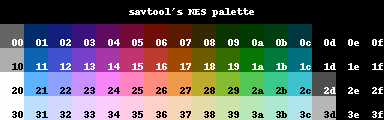
\includegraphics{palette.png}
	\caption{A 2C02 színpalettája}
\end{figure}

\clearpage

\subsection{Paletta indexek}

A $\$3F00 - \$3F1F$ címtartományon található memóriaterületen kerülnek eltárolásra a használatban lévő színek azonosítói. A hardveres limitációk miatt a hátteret 16x16 pixeles cellákra osztották fel. Egy cellán belül kizárólag 4 féle szín fordulhatott elő. Ezeket a 4 színből álló színkombinációkat kissé megtévesztő módon szintén palettáknak nevezik.

\begin{table}[H]
	\centering
	\begin{tabular}{ | l | l | }
		\hline
		Tartomány & Paletta \\
		\hline			
		$ \$3F00 $ & Univerzális háttérszín \\
		$ \$3F01 - \$3F03 $ & 0. háttér paletta \\
		$ \$3F05 - \$3F07 $ & 1. háttér paletta \\
		$ \$3F09 - \$3F0B $ & 2. háttér paletta \\
		$ \$3F0D - \$3F0F $ & 3. háttér paletta \\
		$ \$3F11 - \$3F13 $ & 0. sprite paletta \\
		$ \$3F15 - \$3F17 $ & 1. sprite paletta \\
		$ \$3F19 - \$3F1B $ & 2. sprite paletta \\
		$ \$3F1D - \$3F1F $ & 3. sprite paletta \\
		\hline
	\end{tabular}
	\caption{A paletta RAM struktúrája}
	\label{fig:paletteram}
\end{table}

\subsection{Alakzattáblázat}

A CHR memóriában található két alakzattáblázat az alakzatokat tárolja egy speciális formátumban. Ha az alakzatokat úgy reprezentálnánk, hogy minden pixelre eltárolnánk egy színkódot, akkor pixelenként 6 bitre lenne szükségünk (mivel 55 színkódból választhatunk). Ehelyett pixelenként csak 2 bitet tárolnunk, ami egy 4 színből álló palettán belül azonosít egy színt. Ezzel a megoldással amellett, hogy egyharmadára csökkent a képek mérete, egyben újrafelhasználhatóvá is váltak: a Super Mario Bros. játékban a felhők és bokrok képe ugyanaz, csupán másik palettával kirajzolva.
Egy alakzattáblázat 16x16 darab alakzatot tartalmaz, ebből adódóan a táblázat teljes mérete $16\cdot16\cdot(8\cdot8\cdot2)\div8 = 4096$ bájt.

\begin{figure}[H]
	\centering
	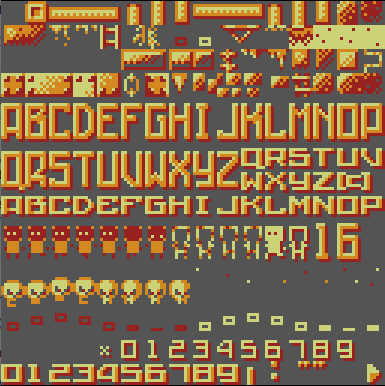
\includegraphics[width=0.45\linewidth,frame]{patt2.png}
	\hspace{5pt}
	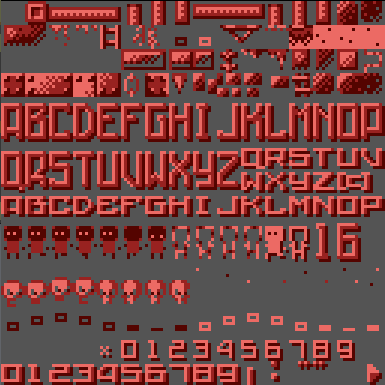
\includegraphics[width=0.45\linewidth,frame]{patt1.png}
	\caption{Az Alter Ego játék 0. mintázat táblája különböző palettákkal kirajzolva}
\end{figure}

\subsection{Rétegek}
A képfeldolgozó két réteget képes kezelni hardveresen, ezek a háttér és a sprite rétegek.
Általában a képkocka azon részei tartoznak a háttérhez, amik ritkán változnak (például feliratok, számlálók, mozdulatlan képek) és a kirajzolásukhoz nem szükséges további transzformáció (eltolás, forgatás). A háttérben az alakzatok 30 sorból és 32 oszlopból álló négyzetrácsot alkotnak (innen ered a NES 256*240 pixeles felbontása).
A háttér rétegben egyesével nem lehet alakzatokat eltolni, csak az egész háttér eltolása lehetséges. A sprite rétegben nagyobb flexibilitás áll rendelkezésre, ugyanis itt egyenként, pixel pontosságú eltolással és tetszőleges elforgatottsággal rajzolhatjuk ki az alakzatokat. A sprite rétegnél legfeljebb 64 alakzat szerepelhet egy képkockán.  

\subsection{Névtáblázat}

A háttér réteg elrendezését a névtáblázatok tárolják. A névtáblázat a háttér 960 darab alakzatcellájának mindegyikéhez eltárolja a cellába rajzolandó alakzat sorszámát az aktív alakzattáblázatban.

\subsection{Attribútum táblák}

Minden névtáblához tartozik egy 64 bájtos attribútumtáblázat, ahol minden bájt egy 4*4 alakzatcellából álló terület palettáit határozza meg. A bájtok 4 darab 2 bites részre vannak felosztva, ahol mindegyik rész egy 2*2 cellából álló terület palettájának sorszámát kódolja el. Ennek a reprezentációnak a következménye, hogy a háttér 4 cellából álló csoportjai mindig egy palettán osztoznak.

\subsection{Háttéreltolás}

A háttéreltolással pixel pontossággal megszabhatjuk, hogy a háttér mely része legyen látható a játékos számára. 

\subsection{OAM}

A sprite réteg elrendezését leíró 256 bájtos memória. 64 darab alakzatról tárol információt, amik a következők:

\begin{compactitem}
	\item X és Y koordináta
	\item Alakzattáblázatbeli sorszám
	\item Elforgatottság
	\item Paletta sorszám
	\item Prioritás a háttérrel szemben
\end{compactitem}


\subsection{Regiszterek}

A CPU és a PPU az alább látható 9 darab egy bájtos regiszter segítségével tud egymással kommunikálni. A regisztereket a CPU a zárójelekben található címeken tudja elérni.

\vspace{0.25cm}

\begin{description}
	\item[CONTROLLER(\$2000):] \hfill
	\begin{compactdesc}
		\item[0-1. bit:] Aktív névtáblázat indexe
		\item[2. bit:] VRAM cím inkrementálási mód
		\item[3. bit:] Aktív alakzattáblázat indexe a sprite rétegnél
		\item[4. bit:] Aktív alakzattáblázat indexe a háttér rétegnél
		\item[5. bit:] Sprite méret (8x8 vagy 8x16 pixel)
		\item[6. bit:] Az emuláció során nem használt bit
		\item[7. bit:] NMI generálása a PPU tétlen periódusának kezdetén
	\end{compactdesc}
	\item[MASK(\$2001):] \hfill
	\begin{compactdesc}
		\item[0. bit:] Szürkeárnyalatos effektus
		\item[1. bit:] Háttér kirajzolása a bal szélső 8 pixel széles oszlopban 
		\item[2. bit:] Sprite-ok kirajzolása a bal szélső 8 pixel széles oszlopban
		\item[3. bit:] Háttér kirajzolása
		\item[4. bit:] Sprite-ok kirajzolása
		\item[5. bit:] Piros szín intenzitásának növelése
		\item[6. bit:] Zöld szín intenzitásának növelése
		\item[7. bit:] Kék szín intenzitásának növelése
	\end{compactdesc}
	\item[STATUS(\$2002):] \hfill
	\begin{compactdesc}
	\item[5. bit:] Sprite túlcsordulás
	\item[6. bit:] Sprite 0 találat
	\item[7. bit:] A PPU a tétlen periódusban van 
	\end{compactdesc}
	\item[OAMADDR(\$2003) és OAMDATA(\$2004):] \hfill \\
	A processzor ezen két regiszter segítségével képes új adatokkal feltölteni az OAM memóriát.
	Az alábbi kódrészlet azt szemlélteti, hogy az \emph{adatok} tömb tartalmát hogyan kell a CPU memóriájából
	az OAM-ba átmásolni egy megadott címtől kezdve.
	\begin{lstlisting}
    OAMADDR := 8 bites OAM cim
    for i in 1..adatok.hossz
    	OAMDATA := adatok[i]
	\end{lstlisting}
	\item[PPUSCROLL(\$2005):] \hfill \\
	Beállíthatjuk vele, hogy a hátteret hány pixellel szeretnénk arrébcsúsztatni (Horizontális tükrözésnél vízszintesen, vertikális tükrözésnél függőlegesen).
	\item[PPUADDR(\$2006) és PPUDATA(\$2007):] \hfill \\
	A névtáblák frissítésére szolgálnak. Hasonlóan kell őket használni, mint az OAMADDR és OAMDATA regisztereket.
	\item[OAMDMA(\$4014):] \hfill \\
	Az OAM memória frissítésének egy alternatív, gyorsabb módja a Direct Memory Access (DMA). Ekkor a processzorban található dedikált hardver másolja át az adatokat egyenesen a CPU RAM-ból az OAM memóriába. A másolás megkezdéséhez annak a memórialapnak a sorszámát kell beírni a regiszterbe, ahol az átmásolandó adatok találhatók.
\end{description}

\subsection{Memóriatérkép}

\begin{table}[H]
	\centering
	\begin{tabular}{ | l | l | }
		\hline
		Tartomány & Paletta \\
		\hline			
		$ \$0000 - \$0FFF $ & 0. Alakzattáblázat \\
		$ \$1000 - \$1FFF $ & 1. Alakzattáblázat \\
		$ \$2000 - \$23FF $ & 0. Névtáblázat \\
		$ \$2400 - \$27FF $ & 1. Névtáblázat \\
		$ \$2800 - \$2BFF $ & 2. Névtáblázat \\
		$ \$2C00 - \$2FFF $ & 3. Névtáblázat \\
		$ \$3000 - \$3EFF $ & A 0-3. névtáblázatok tükrözése \\
		$ \$3F00 - \$3F1F $ & Paletta indexek \\
		$ \$3F20 - \$3FFF $ & Paletta indexek tükrözése \\
		\hline
	\end{tabular}
	\caption{A képfeldolgozó memóriatérképe}
	\label{fig:ppumemmap}
\end{table}

\section{A kirajzolási folyamat}

\subsection{Időzítések}

\subsection{A háttér kirajzolása}

\subsection{Sprite kiértékelés}

\section{Az emulátor megvalósítása}

\subsection{Adatreprezentáció}

\subsection{Monád}

\section{A processzor megvalósítása}

\section{A képfeldolgozó megvalósítása}

\section{Inputkezelés megvalósítása}

\section{A grafikus felhasználói felület}

\section{Interakció a felhasználóval}

\subsection{UML Use-Case diagram}

\section{Tesztelés}




